\documentclass[a4paper, 14pt]{extarticle}
\usepackage{amsmath, amssymb, mathpazo, tikz}

\title{Triangle Centres}

\begin{document}
\maketitle

\subsection*{Centroid}

The three \emph{medians} of a triangle are the lines joining the
vertices with the midpoints of the opposite sides.

The three medians meet at the \emph{centroid}

\begin{center}
  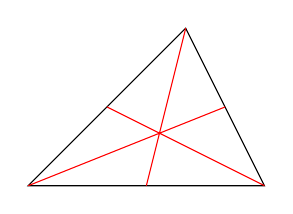
\begin{tikzpicture}
    \draw (0,0) -- (3,0) -- (2,2) -- cycle;
    \draw[red] (1.5,0) -- (2,2) (2.5,1) -- (0,0) (1,1) -- (3,0);
  \end{tikzpicture}
\end{center}

The centroid is the centre of mass of a solid triangle.

\subsection*{Circumcentre}

Any triangle has a \emph{circumscribing circle} or
\emph{circumcircle}, and the centre of that circle is the
\emph{circumcentre}.

\begin{center}
  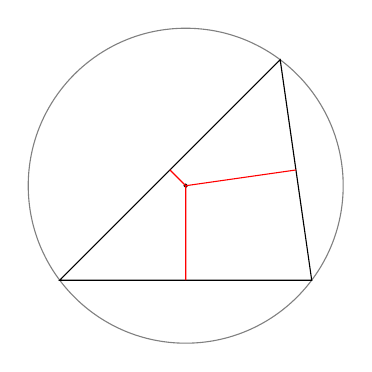
\begin{tikzpicture}
    \draw[gray] (0,0) circle[radius=2];
    \draw[fill=red] (0,0) circle[radius=0.02];
    \draw (1.6,-1.2) -- (-1.6,-1.2) -- (1.2,1.6) -- cycle;
    \draw[red] (0,0) -- (0,-1.2) (0,0) -- (-0.2, 0.2) (0,0) -- (1.4,0.2);
  \end{tikzpicture}
\end{center}

Because the centre of a circles lies on the perpendicular bisector of
any chord, the circumcentre is the intersection of the three
perpendicular bisectors of the edges.

\subsection*{Orthocentre}

Given a triangle, an \emph{altitude} is the line from any vertex that
runs perpendicular to the opposite edge.

\begin{center}
  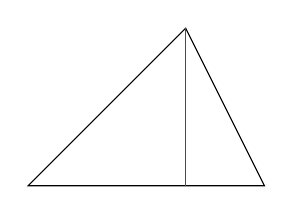
\begin{tikzpicture}
    \draw (0,0) -- (3,0) -- (2,2) -- cycle;
    \draw[red] (2,2) -- (2,0);
  \end{tikzpicture}
\end{center}

The three altitudes also meet at a point, called the \emph{orthocentre}.

If $H$ is the orthocentre of triangle $ABC$, then $A$ is the
orthocentre of triangle $HBC$, and $B$ is the orthocentre of triangle
$AHC$, and $C$ is the orthocentre of triangle $ABH$.

\subsection*{Incentre}

Any triangle has an \emph{inscribed circle} or \emph{incircle}. The
centre of the incircle is the \emph{incentre}.

The incentre of a triangle is the intersection of its three angle
bisectors.

\subsection*{To do\ldots}

\begin{itemize}
\item (JDC will work out how to do the power-of-a-point thing efficiently.)
\item Still got geometry to be going on with.
\item The content above on triangle centres contains other basic stuff
  that could be written up.
\item Continue trying to write functions which encapsulate common bits
  of geometry.
\end{itemize}

\end{document}
